\documentclass{article}


\usepackage{arxiv}

\usepackage[utf8]{inputenc} % allow utf-8 input
\usepackage[T1]{fontenc}    % use 8-bit T1 fonts
\usepackage{hyperref}       % hyperlinks
\usepackage{url}            % simple URL typesetting
\usepackage{booktabs}       % professional-quality tables
\usepackage{amsfonts}       % blackboard math symbols
\usepackage{nicefrac}       % compact symbols for 1/2, etc.
\usepackage{microtype}      % microtypography
\usepackage{lipsum}
\usepackage{graphicx}
\graphicspath{ {./images/} }


\title{Mask Usage Recognition using Vision Transformer with Transfer Learning and Data Augmentation}


\author{
 Hensel Donato Jahja \\
  Faculty of Computer Science\\
  Brawijaya University\\
  Malang, PA 65145 \\
  \texttt{henseldonato@student.ub.ac.id} \\
  %% examples of more authors
   \And
 Novanto Yudistira \\
Faculty of Computer Science\\
  Brawijaya University\\
  Malang, PA 65145 \\
  \texttt{yudistira@ub.ac.id} \\
  \And
 Sutrisno \\
Faculty of Computer Science\\
  Brawijaya University\\
  Malang, PA 65145 \\
  \texttt{trisno@ub.ac.id} \\
  %% \AND
  %% Coauthor \\
  %% Affiliation \\
  %% Address \\
  %% \texttt{email} \\
  %% \And
  %% Coauthor \\
  %% Affiliation \\
  %% Address \\
  %% \texttt{email} \\
  %% \And
  %% Coauthor \\
  %% Affiliation \\
  %% Address \\
  %% \texttt{email} \\
}

\begin{document}
\maketitle
\begin{abstract}
	The COVID-19 pandemic has disrupted various levels of society. The use of masks is essential in preventing the spread of COVID-19 by identifying an image of a person using a mask. Although only 23.1\% of people use masks correctly, Artificial Neural Networks (ANN) can help classify the use of good masks to help slow the spread of the Covid-19 virus. However, it requires a large dataset to train an ANN that can classify the use of masks correctly. MaskedFace-Net is a suitable dataset consisting of 137,016 digital images with 4 class labels, namely Mask, Mask Chin, Mask Mouth Chin, and Mask Nose Mouth. Mask classification training utilizes Vision Transformers (ViT) architecture with transfer learning method using pre-trained weights on ImageNet-21k, with RandAugment. The model training process uses 20 epochs, an Stochastic Gradient Descent (SGD) optimizer with a learning rate of 0.03, a batch size of 64, a Gaussian Cumulative Distribution (GeLU) activation function, and a Cross-Entropy loss function to compare the three architectures of ViT, namely Base-16, Large-16, and Huge-14. Furthermore, the comparison of with and without augmentation and transfer learning are conducted. The results of this study found transfer learning and augmentation using ViT Huge-14 is the best classification. Using this method on MaskedFace-Net dataset, the research reach an accuracy of 0.9601 on training data, 0.9412 on validation data, and 0.9534 on test data. This research shows that training with data augmentation and transfer learning improves classification of the mask usage, even better than convolutional based Residual Network (ResNet).
\end{abstract}


% keywords can be removed
%\keywords{First keyword \and Second keyword \and More}


\section{Introduction}
During the COVID-19 pandemic, the economy, medical resources, and various types of sectors have disrupted the health and development of the affected communities. At the time when COVID-19 first appeared, the two countries most affected (China and South Korea) recommended the use of masks to reduce the spread of coronavirus 2 (SARS-CoV-2) \citep{Feng2020}.
The use of masks was controversial in several countries at the beginning of coronavirus 2 first known. However, previous studies in respiratory diseases such as H1N1 influenza have shown significant results in reducing the spread of the virus by using face masks \citep{Cowling2010}. In addition, research on the risk assessment of the spread of coronavirus 2, has shown that wearing a full-face mask can delay the spread of influenza \citep{Brienen2010}.
People who use masks can reduce virus transmission, but if masks is not properly used, it can increase the risk of spreading coronavirus 2 (World Health Organization, 2020). However, in a study conducted in Japan within its society, only 23.1\% of people used masks properly \citep{Machida2020}. Therefore, supervision of the use of masks is necessary because regions that carry out mandatory mask regulations have seen a decrease in cases infected with coronavirus 2 \citep{VanDyke2020}.

Artificial Neural Networks (ANN) can help classify the usage of the mask through image recognition by learning the extracted feature of various images by processing the images through the layer repeatedly. ANN will deliver the best performance incrementally with the size and uniqueness of the data set \citep{shahinfar2020datasize}. Through some research, we found that Masked Face-Net data set \citep{Cabani2021} is the best choice for this research. The data set consists of 137,016 digital images using masks with 4 class labels: Mask, Mask Chin, Mask Mouth Chin, and Mask Nose Mouth. Each image has a dimension of 1024 by 1024 pixels.
Since the published paper on Gradient-based learning applied to document recognition \citep{lecun1998cnn}, the Convolutional Neural Network (CNN) has become the standard of image recognition. Since then, various multiple papers have been published to beat the predecessor results on data set such as ImageNet \citep{deng2009imagenet}. Almost all the state-of-the-art paper is based on the backbone of convolutional neural networks such as Inception \citep{szegedey2014inception}, VGG \citep{simonyan15vgg}, ResNet \citep{he2015resnet} and the latest EfficientNet \citep{tan2019efficientnet} which beat all the previous CNN architecture. Throughout the years, the trend for image recognition has been going deeper on the layer used in training \citep{alzubaidi2021surveycnn}, which means it requires more computing resources to be used, hence causing an inefficient research in ANN study with a limited resources, another research conducted by \citep{novanto2020} shows that the more layers in an ANN, it will affect the training time, this will adversely affect the efficiency of computational efficiency, especially in large data sets. However, Vision Transformer \citep{Dosovitskiy2020} , another model architecture proven to be faster, and its performance is comparable to EfficientNet while being 5 times faster in computation times. Vision Transformer work by using the attention mechanism used in paper Attention is all you need \citep{Vaswani2017}, by positioning embedded flatten patches of images to attention mechanism and then passed through the multi-layer perceptron layer to classify each class.


Training an ANN might be complicated if we train from scratch. One method that can be applied is to use transfer learning. Transfer learning uses ANN weights, which have previously been trained on larger data set, and applied to data set that have never been used. Using this method can improve accuracy compared to models created from scratch \citep{Barman2019}. The benchmark pre-trained weights used for transfer learning which is usually based on state-of-the-art data set such as ImageNet21k \citep{deng2009imagenet}. ImageNet21k consists of more than 14 million images and 21 thousand categories. The enormous numbers of images and categories will help jump-start the learnable parameter in the training process with immense accuracy to begin.
ANN performance improves concurrently with the size of the data set used in training \citep{alom2019datasetsize}. Data augmentation helps increase the accuracy and quality of data set by modifying the form of the data before being inserted into the model architecture. Furthermore, it improves the performance of deep neural networks (DNN) and thus increases the generalization of model \citep{Wang2016}.

The contributions of our research are:
\begin{enumerate}
	\item Recognition of the usage of the mask is conducted in detail, namely Proper Mask, Mask Chin, Mask Nose Mouth, and Mask Mouth Chin.
	\item We show that the performance of ViT outperforms CNN while the majority of mask classifications are based on CNN backbone.
	\item Data augmentation and transfer learning improve the performance of various ViT models.
	\item ViT model visually shows better attention maps than ResNet via GradCam.
\end{enumerate}


\section{Related Works}\label{related_works}
Research has been conducted to classify masks to stay safe during the COVID-19 pandemic. Solutions to optimize mask usage recognition to prevent the spread of the virus are a hot topic. Research by \cite{Tomas2021} entitled "Incorrect Facemask-Wearing Detection Using CNN with Transfer Learning" uses a crowd data set with 13 categories. A manual label was carried out by a nursing group from the hospital of the Ontinyent, resulting in 3,200 images from 500 users. To help boost the performance of this small data set, the authors compared multiple methods such as data augmentation and transfer learning. They evaluated the results of multiple architectures such as MobileNet \citep{howard2017mobilenets} that have the smallest size footprint of 3.5 million parameters compared to VGG16 \citep{simonyan15vgg} of 134.4 million parameters. VGG16 produces the best accuracy of 0.834 using transfer learning and data augmentation. Although the research results are promising,  \cite{Sarker2021realworldapplications} mentioned that it is needed for deep learning applications to yield at least an accuracy of 0.95 to work correctly in real-life scenarios. Through this research, we believe we can improve the robustness of recognition.

Another research done by \cite{Loey2021maskdetection} used real-world masked face data set (RMFD) \citep{wang2020RMFD} which consists of 5,000 masked and 90,000 unmasked faces of real-world mask usage with similar faces. Labeled Faces in the Wild (LFW) \citep{kawulok2016advances} which consist of 13,000 simulations of masked faces were introduced. Furthermore, they proposed the usage of a hybrid deep transfer learning model, with the ResNet50 (\cite{he2015resnet}) as a features extractor. Finally, the use of Support Vector Machines \citep{Cristianini2008svm} and decision tree \citep{breiman1984decisiiontree} to form an ensemble learning \citep{zhang2012ensemble} perform well with average prediction accuracy of 100\% on RMFD and LFW data set.

Research by \cite{Bosheng2020} with the title "Identifying Facemask-Wearing Condition Using Image Super-Resolution with Classification Network to Prevent COVID-19" uses the Super-Resolution and Classification Networks (SRCNet) architecture, with transfer Learning method capable of achieving up to 98.70\% accuracy. This research inspired our work to utilize transfer learning. Another paper has made annotated data set (\cite{Loey2021NovelDeep}) of Medical Masks Dataset (MMD), which consists of 853 images belonging to 3 categories of mask, without mask, and mask worn incorrectly. This yields much more precise result of 81\% by using YOLOv2 \citep{redmon2015yolo} and ResNet \citep{he2015resnet} feature extraction. The research done by \cite{Li2012annotated} concluded that probabilistic model training with annotated images should perform better than non-annotated images. However, the required number of annotated images in the deep learning research is hard to validate.


\section{Methods and solutions}
\subsection{data set}\label{data_sets}
The related works that we have cited in the previous chapter concluded that we need large resolution and data set size to achieve better accuracy, uniqueness of the images, and perform better in a real-world application.
The data that we used in this study was MaskedFace-Net, \citep{Cabani2021} in which consists of 4 categories of Mask, Mask Chin, Mask Nose Mouth, and Mask Mouth Chin. The total of this data set is 133.738 images with 1024x1024 resolution. The data set is widely sparse and non-biased through one category, so we believe this is the best data set we can use in this research. The data set is based on Flicker data set \citep{karras2018gan} which is leveraged to be training data for generative adversarial network (GAN) in image generation. Moreover, the author of MaskedFace-Net uses facial landmark detections to detect facial features and mask-to-face mapping to add a mask on the face. Fig. \ref{mfn_fig} shows samples from MaskedFace-Net. From left to right, we have Mask category with mask usage that covers the nose,mouth, and chin; Mask Chin category in the second column covered only the chin part of the face; Mask Mouth Chin, which covered the mouth and the chin of the face, and; Mask Nose Mouth, with mask usage that covered only the nose and the mouth or face. Although it consists of only four categories, the data set is detailed, large, sparse, and thus capable of being used in various GAN\citep{karras2018gan}.
\begin{figure}[!b]
	\centering
	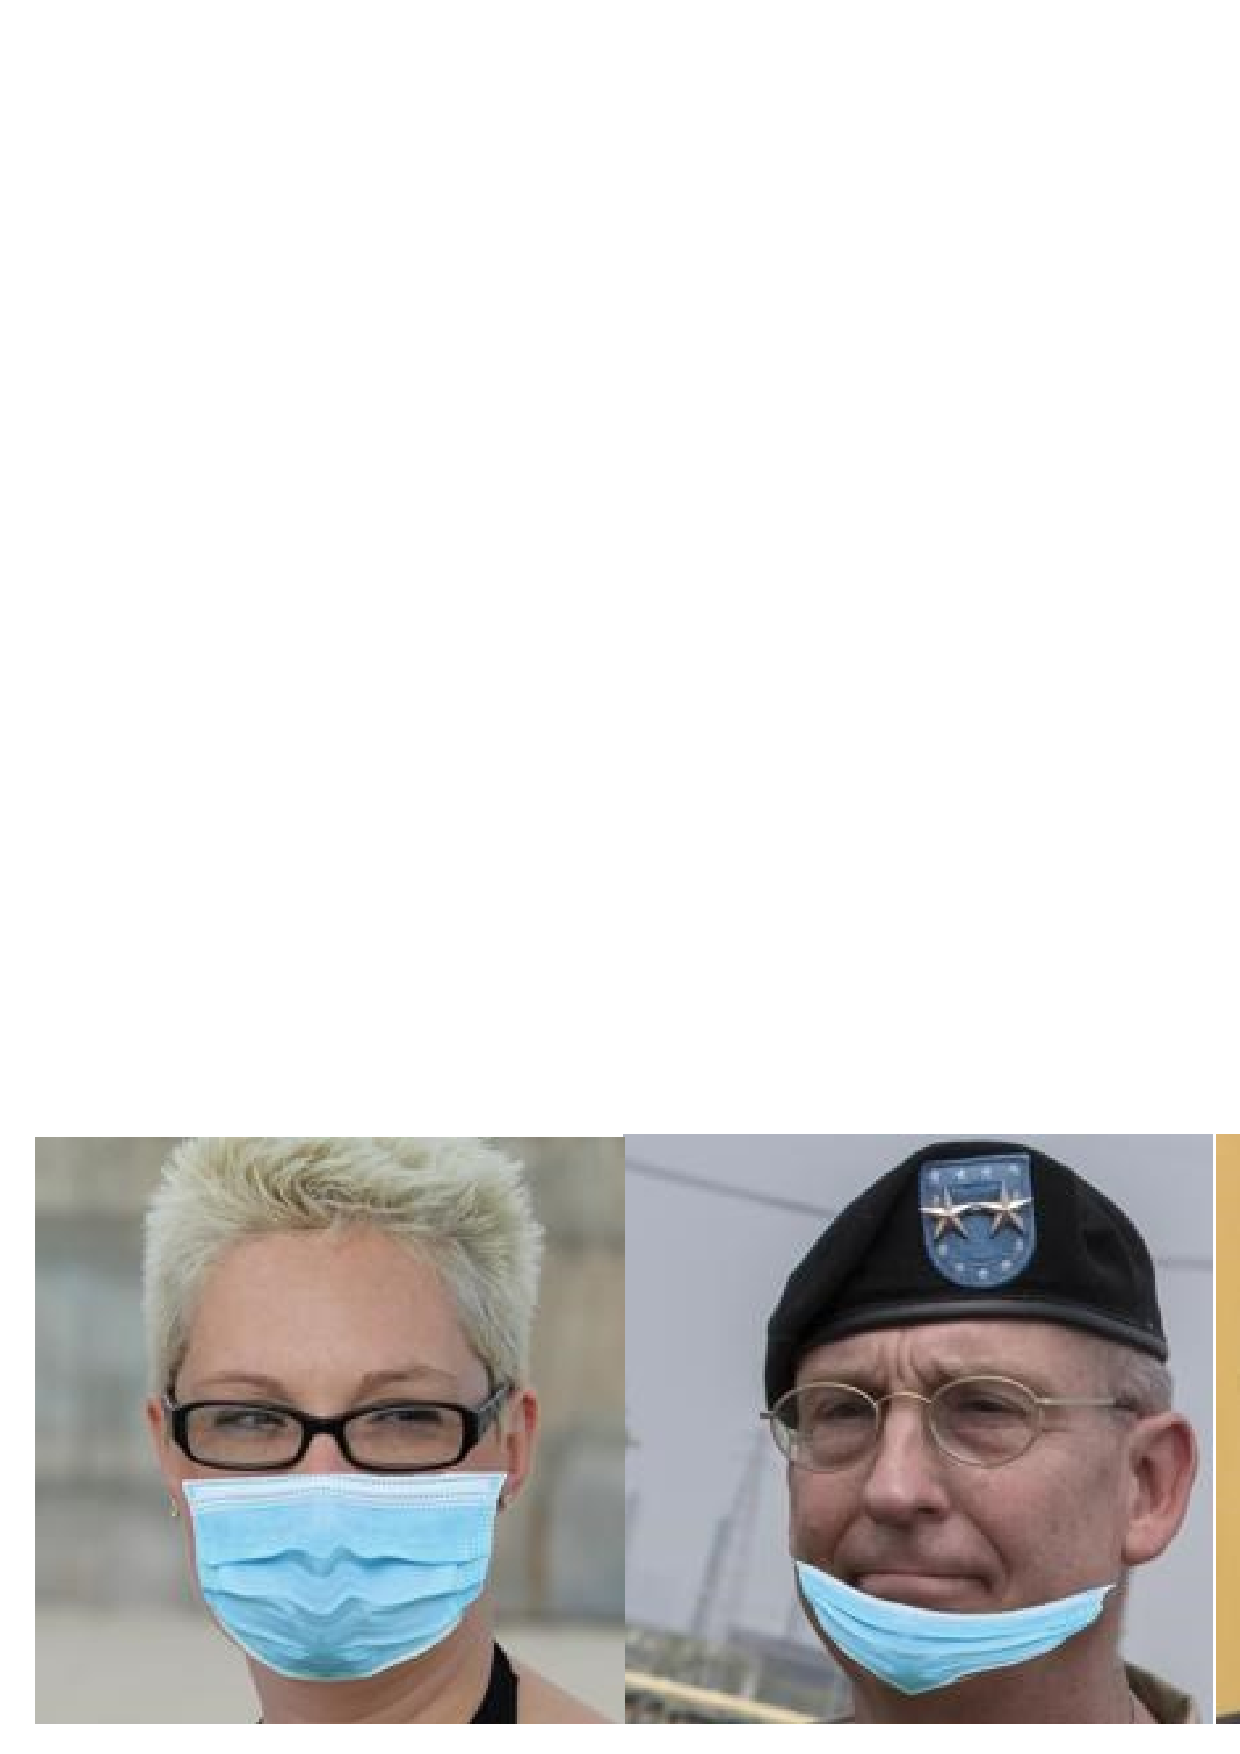
\includegraphics[scale=.3]{mfn.pdf}
	\caption{MaskedFace-Net sample.}
	\label{mfn_fig}
\end{figure}


\subsection{Vision transformers}\label{vision_transformers}
Transformer was introduced in 2017 with a journal entitled Attention Is All You by \cite{Vaswani2017}, to overcome problems in the Recurrent Neural Network (RNN) \citep{Hopfield1982rnn} and Long Short Term Memory (LSTM) \citep{hocreiter1997lstm} models. Both models have problems with loss gradients and long training times in the case of Natural Language Processing (NLP). For years, image classification tasks have always used CNN \citep{lecun1998cnn} as the backbone of the architecture. However, in a 2020 \cite{Dosovitskiy2020}, it was discovered that Transformers could be used for image classification research, with five times faster in computation time than the latest state of the art convolutional architecture while keeping the accuracy head to head.


ViT are not the usual image classification architecture we have seen before. Fig. \ref{ViT Fig.} is an overview of the Vision Transformer model. Images are split into several parts based on the number of patches that have been declared after going through the process of splitting a 2-dimensional digital image. It is necessary to change the 2-dimensional digital image into a 1-dimensional vector, Eq. \ref{lp_eq} is a formula for changing a 2-dimensional image into a 1-dimensional vector, where \textit{H},\textit{W}, is the resolution of the image, and \textit{C}  and C is the channels numbers, which will be converted into a
\begin{math}
	R^{N x\left(P^{2} \cdot C\right)}
\end{math} where $P$ is the number of patches and $N=HW/P^2$. After that, the embedding results will pass through the transformers encoder.
ViT encoder behaves just like the encoder mechanism. We found Transformers for natural language processing task on the paper Attention is All You Need \citep{Vaswani2017} that it takes an embedded input. Then it is processed through layer normalization \cite{ba2016layer} which uses the distribution of the summed input to a neuron over a mini-batch of training cases. Computing mean and variance, which are then used to normalize the summed input, gives a huge time advantage compared to batch normalization. The multi-head self-attention is needed to capture the image's critical part. Eq. \ref{attn_eq} shows the equation for attention, where $Q$ is the query or the pure input value from the embedding, $K$ is the permutation of the input, and $V$ is the scaled dot product from $Q$ and $K$ with softmax activation. Multi-head attention contains the concatenation of multi self-attention, as seen in Eq. \ref{mha_eq} where the number of heads will be multiplied with the $W^{O}$ value. This gives the transformers encoder the best feature extraction to attend the important part. Unlike the other works that we have seen in Section \ref{related_works}, most of the feature extraction uses ResNet \citep{he2015resnet} feature extractor to obtain the most critical part of the images. However, the self-attention on transformers encoder \citep{Dosovitskiy2020} will result well enough without another feature extraction. The last layer of transformers encoder is a simple multilayer perceptron, with each output is based on the category that we have defined in our data set, which in our case is four, with the activation of the multilayer perceptron utilizaing GeLU \citep{hendrycks2016gelu}.

\begin{equation}
	x \in R^{H x W x C} \rightarrow x_{p} \in R^{N x\left(P^{2} . C\right)}
	\label{lp_eq}
\end{equation}

\begin{equation}
	AttentionHead(Q, K, V)=softmax(\frac{QK^T}{\sqrt{d_k}})V
	\label{attn_eq}
\end{equation}

\begin{equation}
	MultiHead(Q, K, V) = Concat(AttentionHead_1, ..., AttentionHead_n)W^O
	\label{mha_eq}
\end{equation}

\begin{figure}[!b]
	\centering
	\includegraphics[scale=.35]{vit_archi.pdf}
	\caption{ViT Model Overview.}
	\label{ViT Fig.}
\end{figure}

\subsection{Data augmentation}
The classification results in the ANN get better when using a larger dataset \citep{shahinfar2020datasize} because the ANN learns from every pixel in a digital image can be obtained using the Data Augmentation process. Data augmentation is a process in digital image processing, which augmentation changes the digital image in such a way, and the digital neural network will study the augmentation of the digital image as a new digital image \citep{Wang2016},  Usage of augmentation can also be seen in paper by \cite{fadhil2020}  which shows the use of augmentation has an effect on training outcomes in an ANN, by showing higher accuracy and lower loss values in the training process, because augmentation can help ANN recognize patterns. There is much research in data augmentation methods to help the performance of ANN training. The latest state of the art is AutoAugment \citep{cubuk2018autoaugment} which applies augmentation of random choices on batch images. AutoAugment works by using the searching algorithm controller Recurrent Neural Network, samples sum of data, and searching the probability of operation using the best result. The disadvantage of AutoAugment is that the process takes much time, especially in large data set. There is a RandAugment \citep{cubuk2019randaugment} solution that eliminates the search for the best augmentation in a phase so that the computation process is fast. By eliminating the search space for the base algorithm to classify the best results and using randomly distributed application augment on the whole data set, the RandAugment method reduce the search space from $10^{32}$ to $10^2$. Although it is much faster than AutoAugment, RandAugment yields the same accuracy results as the latest state-of-the-art, and it does not linearly increase the search space to the data set sizes.

% \begin{figure}[!b]
%   \centering
%   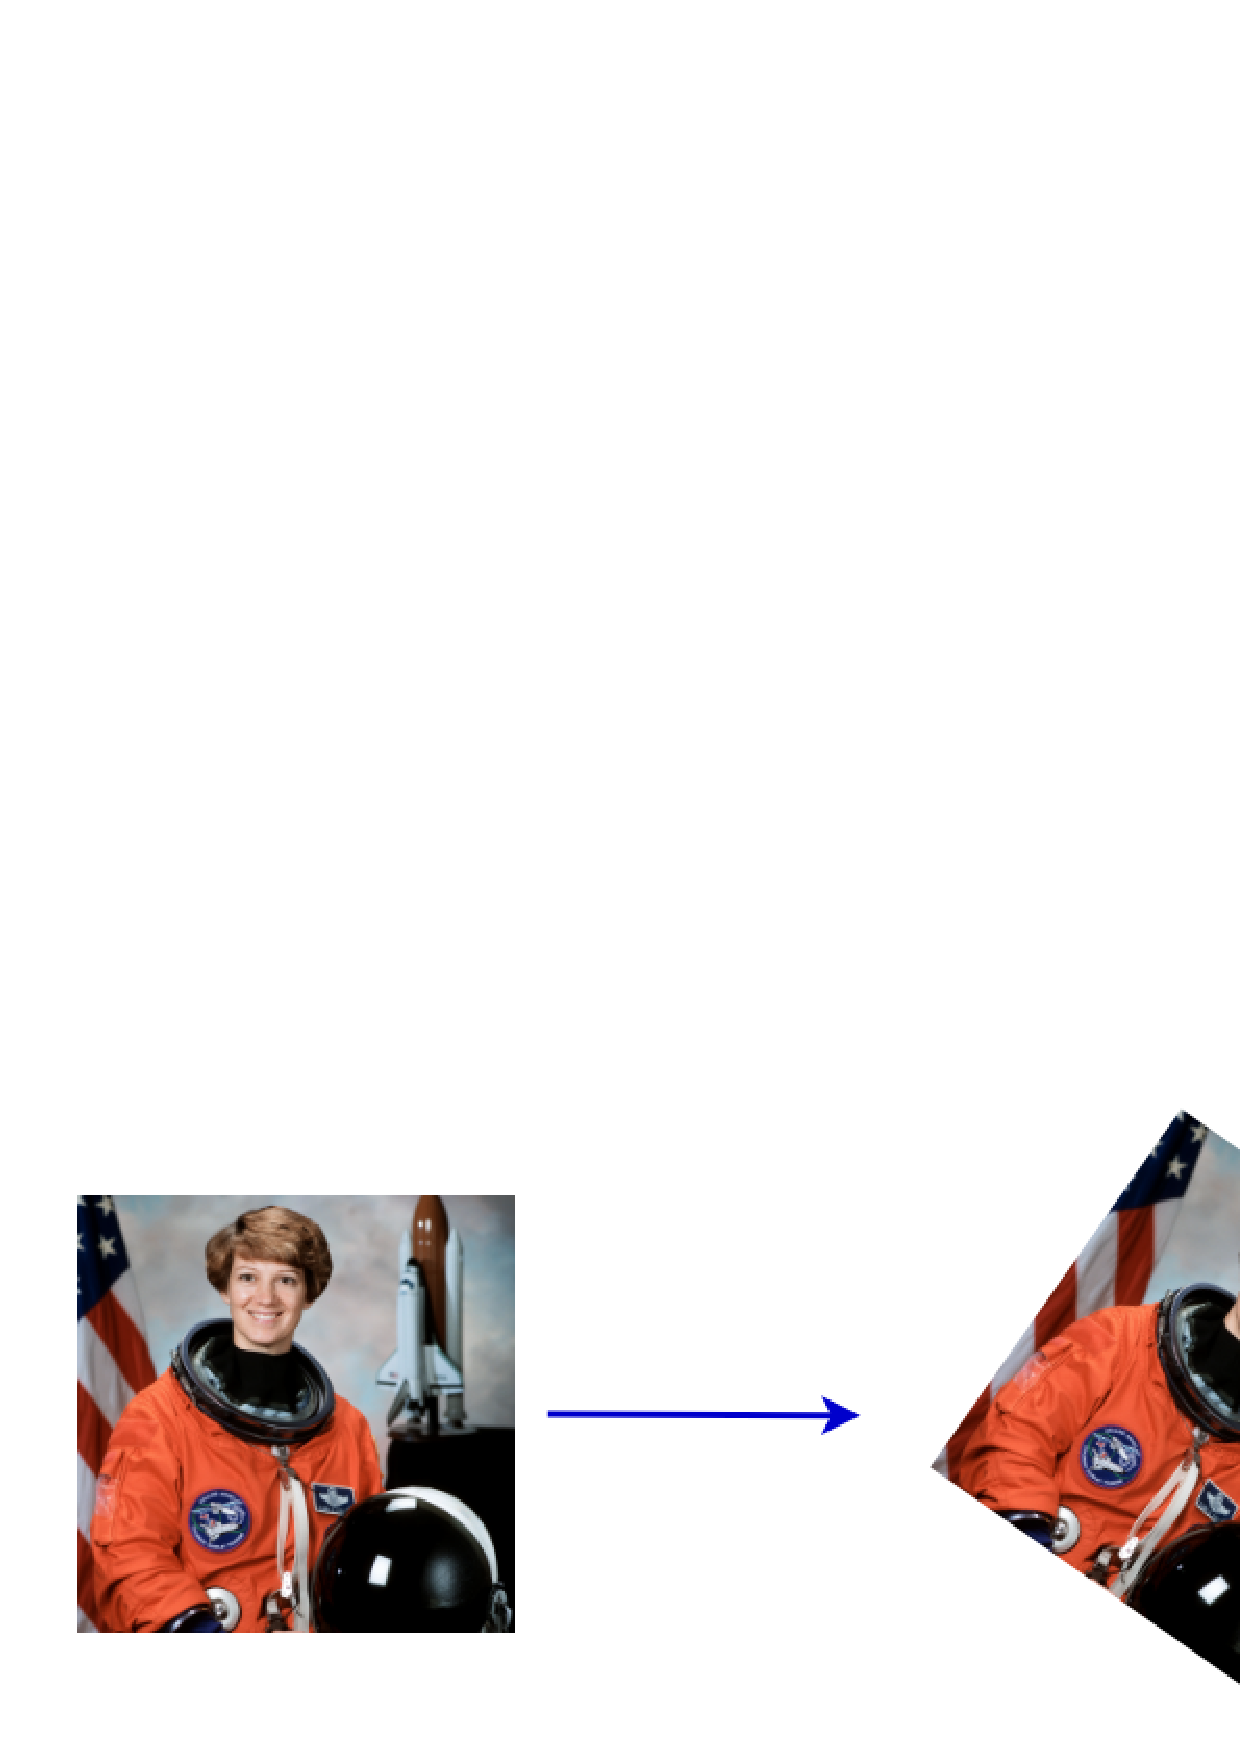
\includegraphics[scale=0.3]{augment.pdf}
%   \caption{Illustration of augmentation \citep{Vasilev2019}.}
%   \label{augment_fig}
% \end{figure}

\subsection{Transfer learning}
The Vision Transformer architecture works best if the architecture has been trained using multiple data set first before being implemented on other data set \citep{Dosovitskiy2020}. The process of training the architecture and getting the weights on each neuron, and implementing it to another data set is called transfer learning. Transfer Learning will work well if the data set used in a transfer learning process has similarities, both from class, type of digital image to digital image resolution. However, the most influential factor on the success of transfer learning is the amount and diversity of data \citep{Weiss2016}. Therefore, this research will use a transformer vision architecture that has been trained on the ImageNet \citep{deng2009imagenet} data set, which is a data set containing 14,197,122 annotated images according to the WordNet hierarchy \citep{Russakovsky2015}.

\subsection{Gradient-weighted class activation mapping (grad-cam)}
Every application in ANN relied on human niche expertise to implement throughout the years. However, the Explainability and comprehensibility of AI are necessary to be deployed in real-world domains because the user needs to understand the system works. Thus it can be adequately tested and referred \citep{yampolskiy2019unexplainable}.
\cite{Selvaraju2020gradcam} proposed a technique for making ANN more explainable. Every training process in ANN needs a gradient to compute the updated weights. Gradient-weighted Class Activation Mapping uses this acquired gradient to produce a coarse localization map by highlighting the critical regions of an image on the last layer convolutional block.
ViT work differently in that the architecture does not use any convolutional block. Instead, we will treat the last layer of the attention block that is not affected by token addition. Eq. \ref{pre-Gradcam Equation}  shows the computation of $w_k^{\left(c\right)}$ with the $H$ as the height of the image, $W$ represent the width of the image. This calculation is needed to sum up the matrix from the chosen layer gradient. Eq. \ref{Gradcam Equation} will multiply the matrix results from \ref{pre-Gradcam Equation} and the dot product of linear product with the input and output images. Finally, ReLU \citep{agarap2018relu} activation, which will return 0 on the value that less than 0  is utilized. This activation will eliminate unnecessary gradient to focus only on the most important part of the gradient mapping on the image.

\begin{equation}
	w_k^{\left(c\right)}=\frac{1}{H\cdot W}\sum_{i=1}^{H}\sum_{j=1}^{W}\frac{\partial Y^{\left(c\right)}}{\partial A_k\left(i,j\right)}
	\label{pre-Gradcam Equation}
\end{equation}

\begin{equation}
	L_{Grad-CAM}^{\left(c\right)}\left(x,y\right)=ReLU\left(\sum_{k}{w_k^{\left(c\right)}A_k\left(x,y\right)}\right)
	\label{Gradcam Equation}
\end{equation}
\subsection{Model training}\label{model_training}
% 		The hardware specification that will be used are reproducible we will be using RTX 8000, Intel(R) Xeon(R) Gold 6230R, RAM 255 GiB
There are various configurations for the Vision Transformer architecture. Constant hyperparameters will be set in training to prevent bias in the test results of each configuration. In this research, we will keep the same setup that  \cite{Dosovitskiy2020} used in the original ViT research. The hyperparameters used for fine-tuning are batch size of 64, a learning rate of 0.03, epochs of 20, loss function of Cross-Entropy \citep{zhang2018crossentropy}, optimizer Stochastic Gradient Descent, and  GeLU \citep{hendrycks2016gelu} activation. For this research, we split the training, validation, and test data set the size of 80\%, 10\%, and 10\%, respectively, from the whole data set of MaskedFaceNet \citep{Cabani2021}. The use of transfer learning from pre-trained weights that have been trained on ImageNet21K \citep{deng2009imagenet}, and augmentation method of RandAugment \citep{cubuk2019randaugment}.

\section{experimental results}

\subsection{Comparing Size of ViT}
Defined variants of ViT can be seen in Table \ref{vit_variants} with ViT base 16 consist of 16x16 patches, 12 layers of transformers encoder, 768 hidden sizes, 3072 of multilayer perceptron in the transformers encoder, 12 attention heads, and sum of parameters of 86 millions. ViT large 16 consists of 16x16 patches, 24 layers of transformers encoder, 1024 hidden size, 4096 of multilayer perceptron in the transformers encoder, 16 attention heads, and the sum of parameters of 307 million. ViT huge 14 consists of 14x14 patches, 32 layers of transformers encoder, 1280 hidden size, 5120 of multilayer perceptron in the transformers encoder, 16 attention heads, and the sum of parameters of 632 million.
We will discuss the effect of architectural size on the accuracy of training, validation, and test data. Table \ref{size_acc_table} shows the training results from 20 epochs, and the highest accuracy value will be taken for each architecture. The results show that the vision transformer huge 14 yields the best results for all data set parts, with an impressive accuracy of 0.93 on the test set. Meanwhile, the transformers large 16 has the worse performance out of the three variants, despite having more than three times the size parameters of ViT base 16.


% 		Table shows the test results on the Vision Transformer Base 16, Vision Transformer Large 16, and Vision Transformer Huge 14 architectures. Fig. \ref{size_acc_fig} shows the training accuracy and validation accuracy for the three architectures.

\begin{table*}[!b]
	\caption{ViT variants.}
	\label{vit_variants}
	\centering
	\begin{tabular}{p{4cm}|p{1.2cm}p{1.2cm}p{1.2cm}p{1.2cm}p{1.2cm}p{1.2cm}}
		% \begin{tabular}{p{3.5cm}|p{2cm}p{2}p{2cm}}
		%%\hline
		Model & Patches & Layers & Hidden Size & MLP size & Heads & Num. of Params \\
		\hline
		Vision transformer base 16 &
		16 &
		12 &
		768 &
		3072 &
		12 &
		86 Mil.\\
		%%\hline
		Vision transformer large 16 &
		16 &
		24 &
		1024 &
		4096 &
		16 &
		307 Mil.\\
		%%\hline
		Vision transformer huge 14 &
		14 &
		32 &
		1280 &
		5120 &
		16 &
		632 Mil.
		%%\hline
	\end{tabular}
\end{table*}

The results of the ViT architecture training and validation epoch by epoch can be seen in Fig. \ref{size_acc_fig}. It can be seen that the highest accuracy value was obtained by the ViT huge 14 architecture at epoch 20 with an accuracy of 0.805519. A significant difference compared to other architectures, namely ViT base 16 of 0.772179, which was obtained in the 14th epoch. Finally, ViT large 16 of 0.717461 were obtained in the 19th epoch. The validation results for each ViT architecture did not differ much from the training results. In this case, the ViT huge 14 got the highest accuracy in the 19th epoch with a value of 0.816742. This is higher than the ViT base 16 architecture of 0.773756, which was obtained at the 13th epoch, and the ViT large 16 architecture of 0.749623 obtained at the 20th epoch. The test results of the test data show that the ViT huge 14 architecture is very high compared to Another ViT architecture is 0.934586.

\begin{table*}[!b]
	\caption{Accuracy of different ViT size}
	\label{size_acc_table}
	\centering
	\begin{tabular}{p{4cm}|p{2cm}p{2cm}p{2cm}}
		% \begin{tabular}{p{3.5cm}|p{2cm}p{2}p{2cm}}
		%%\hline
		Model & Train & Validation & Test \\
		\hline
		Vision transformer base 16 &
		0.772179 &
		0.773756 &
		0.818045 \\
		%%\hline
		Vision transformer large 16 &
		0.717461 &
		0.749623 &
		0.766917 \\
		%%\hline
		Vision transformer huge 14 &
		\textbf{0.805519} &
		\textbf{0.816742} &
		\textbf{0.934586} \\
		%%\hline
	\end{tabular}
\end{table*}

\begin{figure}[!b]
	\centering
	
\includegraphics[scale=.02]{size_acc.pdf}
	\caption{Accuracy of different ViT in 20 epochs}
	\label{size_acc_fig}
\end{figure}

\subsection{Effects of augmentation on accuracy}
Random Augment Policy will be used on training and validation data set and based on the results of previous research. The ViT huge 14 architecture will be used because this architecture yields the best accuracy on training, validation, and test set. In this test, we will compare the results augmentation, and without augmentation, on training data with the same setup we define at Subsection \ref{model_training}

From the test results on the accuracy of augmented and non-augmented data can be seen in Table \ref{aug_acc_table}, the data with augmentation got higher accuracy, with a value of 0.816821 for training data, 0.82167 for validation data, compared to data without augmentation of 0.805519 for training data, and 0.816742 for validation data. A comparable accuracy is obtained in the test data, which is 0.934586. The augmentation results on all set yield much better accuracy than without augmentation. Fig. \ref{aug_acc_fig} shows epoch by epoch accuracy on augmentation applied ViT, and it can be seen that those ViT with augmentation yield the best results on the 13th epoch, compared to training without the augmentation that yields the best results on the 20th epoch. Validation on both augmented and non-augmented data set yields the same results as the training data set. We concluded that augmentation on the training converges faster than without augmentation.

\begin{table*}[!b]
	\caption{Effects of augmentation on ViT huge 14}
	\label{aug_acc_table}
	\centering
	\begin{tabular}{p{4cm}|p{2cm}p{2cm}p{2cm}}
		%%\hline
		Model & Train & Validation & Test \\
		\hline
		Augmentation &
		0.816821 &
		0.821267 &
		0.934586 \\
		%%\hline
		Without augmentation &
		\textbf{0.805519} &
		\textbf{0.816742} &
		\textbf{0.934586} \\
		%%\hline
	\end{tabular}
\end{table*}

\begin{figure}[!b]
	\centering
	
\includegraphics[scale=.02]{aug_acc.pdf}
	\caption{Impacts of augmentation on accuracy}
	\label{aug_acc_fig}
\end{figure}


\subsection{Impacts of transfer learning method}

In testing the effect of pretrained weights, we will compare the results of using pretrained weights without using pretrained weights. In this subsection, we will use pretrained weights that have been trained using the ImageNet21K dataset on the ViT huge 14 architecture, with training and validation data set that has been augmented,
In testing the results of accuracy against the use of pretrained weights and without using pretrained weights can be seen at \ref{tl_acc_table} which shows the best accuracy accross all 20 epochs that it has been trained. It was found that using pretrained weights got higher results with accuracy in training data of 0.960068, validation data of 0.941176, and on test data of 0.953383, compared to without using pretrained weights with accuracy on training data of 0.816821, validation data of 0.82167, and test data of 0.934586. Fig. \ref{tl_acc_fig} shows epoch by epoch of the training and validation phase. It can be seen that the model that uses pretrained weights starts the training with much better accuracy compared to without the usage of pre-trained weights. From epoch 13th there is a considerable drop in accuracy caused by gradient loss. It did not happen in the model with the pretrained weights. From these results, we can conclude that the usage of pretrained weights performs much better than without it.

\begin{table*}[!b]
	\caption{Impacts of transfer learning on ViT huge 14}
	\label{tl_acc_table}
	\centering
	\begin{tabular}{p{4cm}|p{2cm}p{2cm}p{2cm}}
		%%\hline
		Model & Train & Validation & Test \\
		\hline
		With Transfer Learning &
		\textbf{0.960068} &
		\textbf{0.941176} &
		\textbf{0.953383}\\
		%%\hline
		Without Transfer Learning &
		0.816821 &
		0.821267 &
		0.934586 \\
		%%\hline
	\end{tabular}
\end{table*}

\begin{figure}[!b]
	\centering
	
\includegraphics[scale=.02]{tl_acc.pdf}
	\caption{Impacts of transfer learning on accuracy}
	\label{tl_acc_fig}
\end{figure}

\subsection{Comparisons with baselines}
After carrying out various experiments on augmentation and pretrained weights, it can be seen that the use of augmentation and pretrained weights simultaneously can increase accuracy and reduce losses in training, validation, and testing. Therefore, experiments using augmentation and pretrained weights will be carried out on all existing architectures and the residual network architecture as a benchmark in this study.


In testing each architecture can be seen on \ref{all_acc_table}, it was found that by using pretrained weights and augmentation on the data, it was found that the ViT large 16 architecture had the highest accuracy value in the training data of 0.986909, and in the validation data of 0.960030. However, in the test data, it was found that the architecture ViT huge 14 has an accuracy value of 0.953383, compared to the value of ViT of 0.928571, which shows that there is overfitting in the architecture of ViT large 16. Fig. \ref{all_acc_fig} shows the 20 epoch training of all architecture. It can be seen that from the train and validation plots, that ResNet \citep{he2015resnet} get inconsistent results in validation and training, such as epoch 18th, where there is a huge drop in accuracy caused by loss of gradient.

\begin{table*}[!b]
	\caption{Impacts of augmentation and transfer learning}
	\label{all_acc_table}
	\centering
	\begin{tabular}{p{4.5cm}|p{2cm}p{2cm}p{2cm}}
		%%\hline
		Model & Train & Validation & Test \\
		\hline
		ViT Base 16 &
		0.963929 &
		0.944947 &
		0.820301\\
		%%\hline
		ViT Large 16 &
		\textbf{0.986909} &
		\textbf{0.96003}	&
		0.928571\\
		%%\hline
		ViT Huge 14 &
		0.960068 &
		0.941176 &
		\textbf{0.953383} &
		%%\hline
		ResNet 50 &
		0.672797 &
		0.521005 &
		0.553454 &
		%%\hline
		ResNet152 &
		0.792082 &
		0.697393&
		0.797244 &
		%%\hline
	\end{tabular}
\end{table*}

\begin{figure}[!b]
	\centering
	
\includegraphics[scale=.02]{all_acc.pdf}
	\caption{Impacts of augmentation and transfer learning on accuracy}
	\label{all_acc_fig}
\end{figure}


\subsection{Confusion matrix}
The best test was obtained by ViT huge 14 using pretrained weights and augmentation. Table \ref{cm_table} is the result of the confusion matrix on the test data. These tests show that the ViT huge 14 with augmentation and pretrained weights can classify each class well. The Mask class prediction accuracy is 0.938462, Mask Chin is 0.761905, Mask Mouth Chin is 0.862682, and Mask Nose Mouth is 0.725. The results of incorrectly presenting the usage seem low, with the highest one being Mask Nose Mouth class classified as Mask with 0.275.


\begin{table*}[!b]
	\caption{Confusion matrix on every class}
	\label{cm_table}
	\centering
	\begin{tabular}{p{2.6cm}|p{2.6cm}p{2.6cm}p{2.6cm}p{2.6cm}}
		%\hline
		% \multicolumn{1}{|c|}{\hspace{2.5cm}} &
		% \multicolumn{4}{c|}{Actual class} \\%\hline
		\hspace{2.5cm} & Mask & Mask Chin & Mask Mouth Chin & Mask Nose Mouth \\
		\hline
		Mask &
		0.967543 &
		0.000000 &
		0.012365 &
		0.020093 \\
		%\hline
		Mask Chin &
		0.000000 &
		0.925926 &
		0.074074 &
		0.000000 \\
		%\hline
		Mask Mouth Chin &
		0.061990 &
		0.032626 &
		0.890701 &
		0.014682 \\
		%\hline
		Mask Nose Mouth &
		0.162791 &
		0.000000 &
		0.023256 &
		0.813953 \\
		%\hline
	\end{tabular}
\end{table*}


\subsection{Grad-Cam Results}
GradCam \citep{Selvaraju2020gradcam} calculations require a gradient on a layer so that the focus of a layer is obtained. In ViT, we will use the gradient of the last attention layer in the architecture to find where the important parts are in an image. We will use the last convolutional gradient layer for the residual network architecture. Based on Table \ref{all_acc_fig} ResNet152  \citep{he2015resnet} performs better than ResNet50, which we will use as comparison with ViT Huge 14, as a comparison. Fig. \ref{mask} is the result of Grad-Cam for the Mask Chin class. In the visualization, it can be seen that vision transformer focuses on the entire face area except for the position of the mask on the chin.
On the other hand, ResNet152 only focuses on the life and mouth. Fig. \ref{mask_mouth_chin} is the Grad-Cam result of the Mask Mouth Chin class. It can be seen that the ViT focus the gradient on the part of the face without a mask. Meanwhile, ResNet152 does not focus the gradient on any face part. Fig. \ref{mask_nose_mouth} is the Grad-Cam result of the Mask Nose Mouth class. It can be seen that the gradient ViT focus more on the mask and looks more precise than ResNet152. Fig. \ref{mask_nose_mouth} Grad-Cam against the Mask class shows a significant comparison, ViT, focusing on the part of the face that does not wear a mask, while ResNet152 focuses the gradient on the part of the face that wears a mask.

\begin{figure}[!b]
	\centering
	
\includegraphics[scale=.015]{mask.pdf}
	\caption{Grad-Cam on mask class}
	\label{mask}
\end{figure}

\begin{figure}[!b]
	\centering
	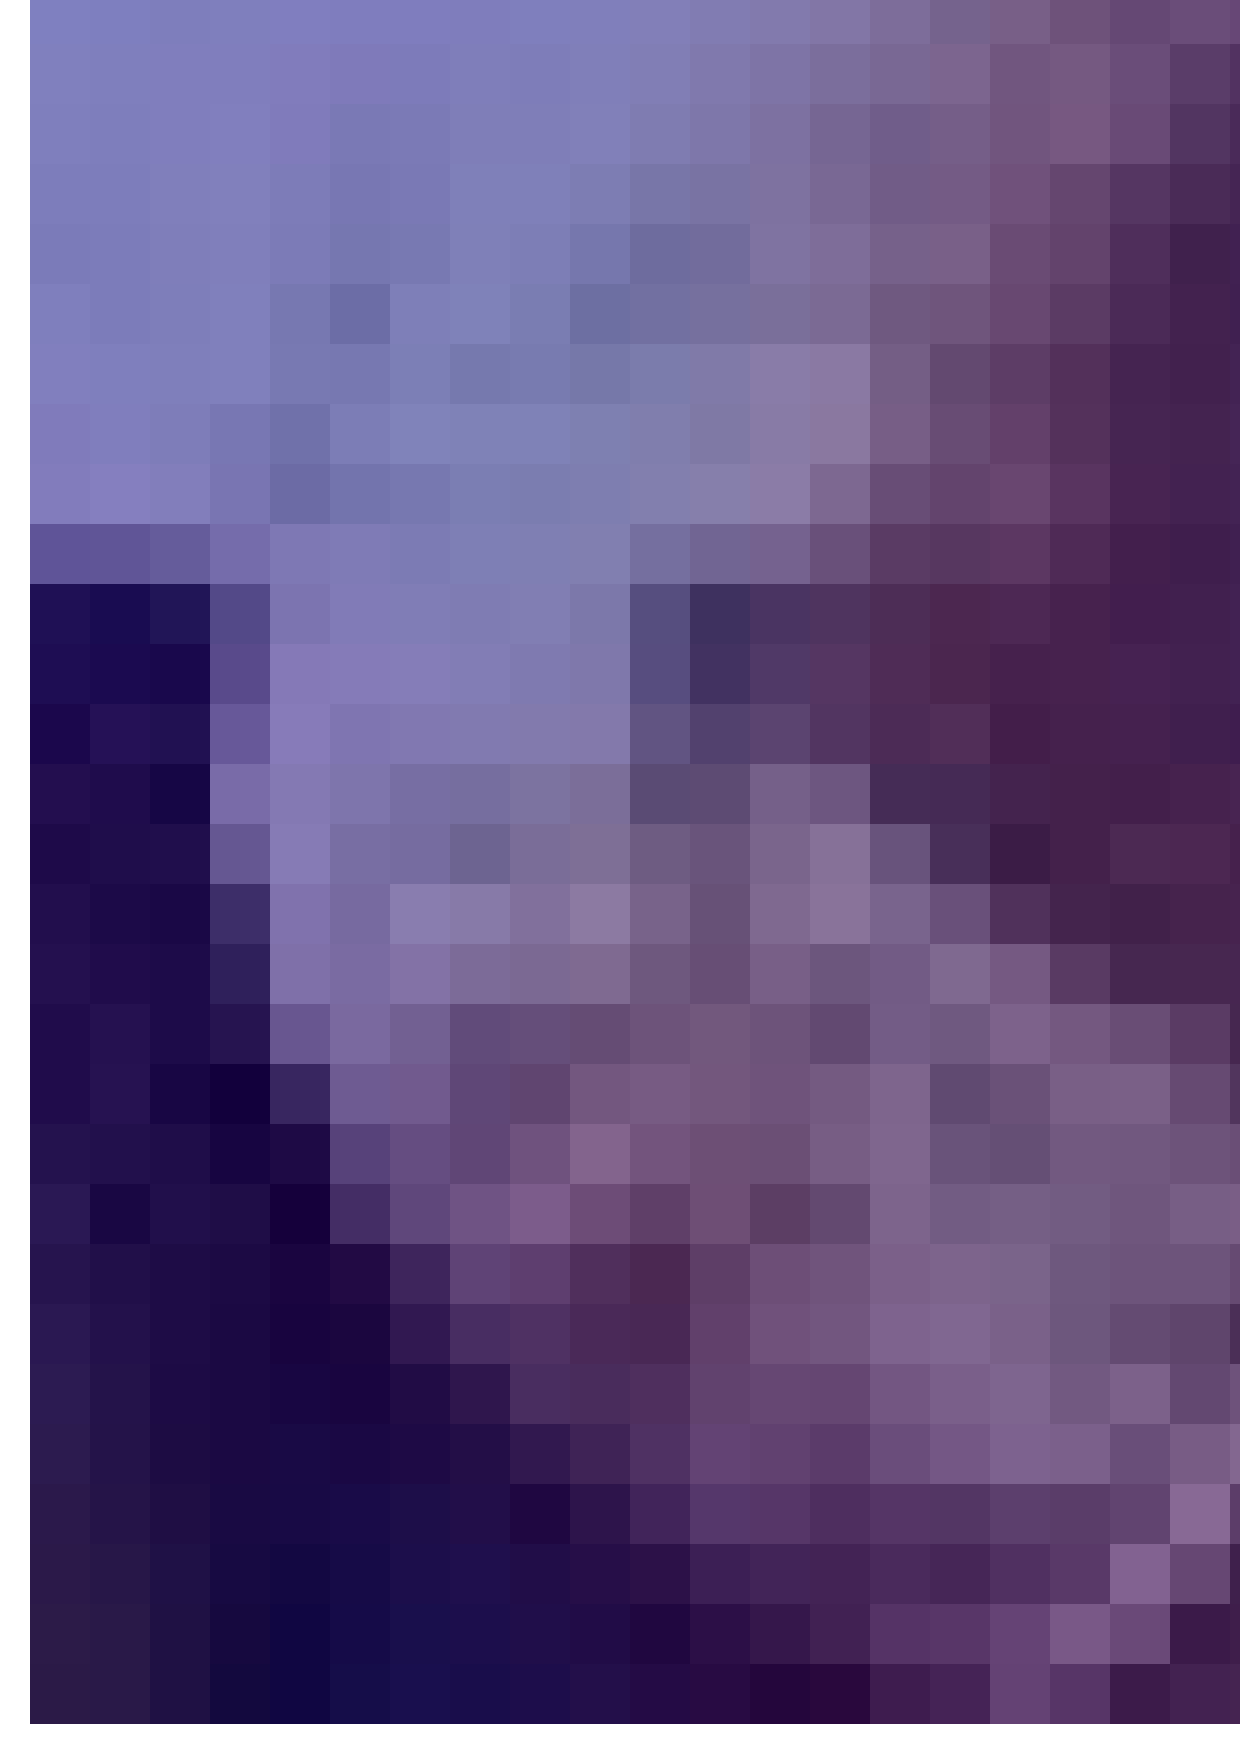
\includegraphics[scale=.015]{mask_mouth_chin.pdf}
	\caption{Grad-Cam on mask mouth chin class}
	\label{mask_mouth_chin}
\end{figure}


\begin{figure}[!b]
	\centering
	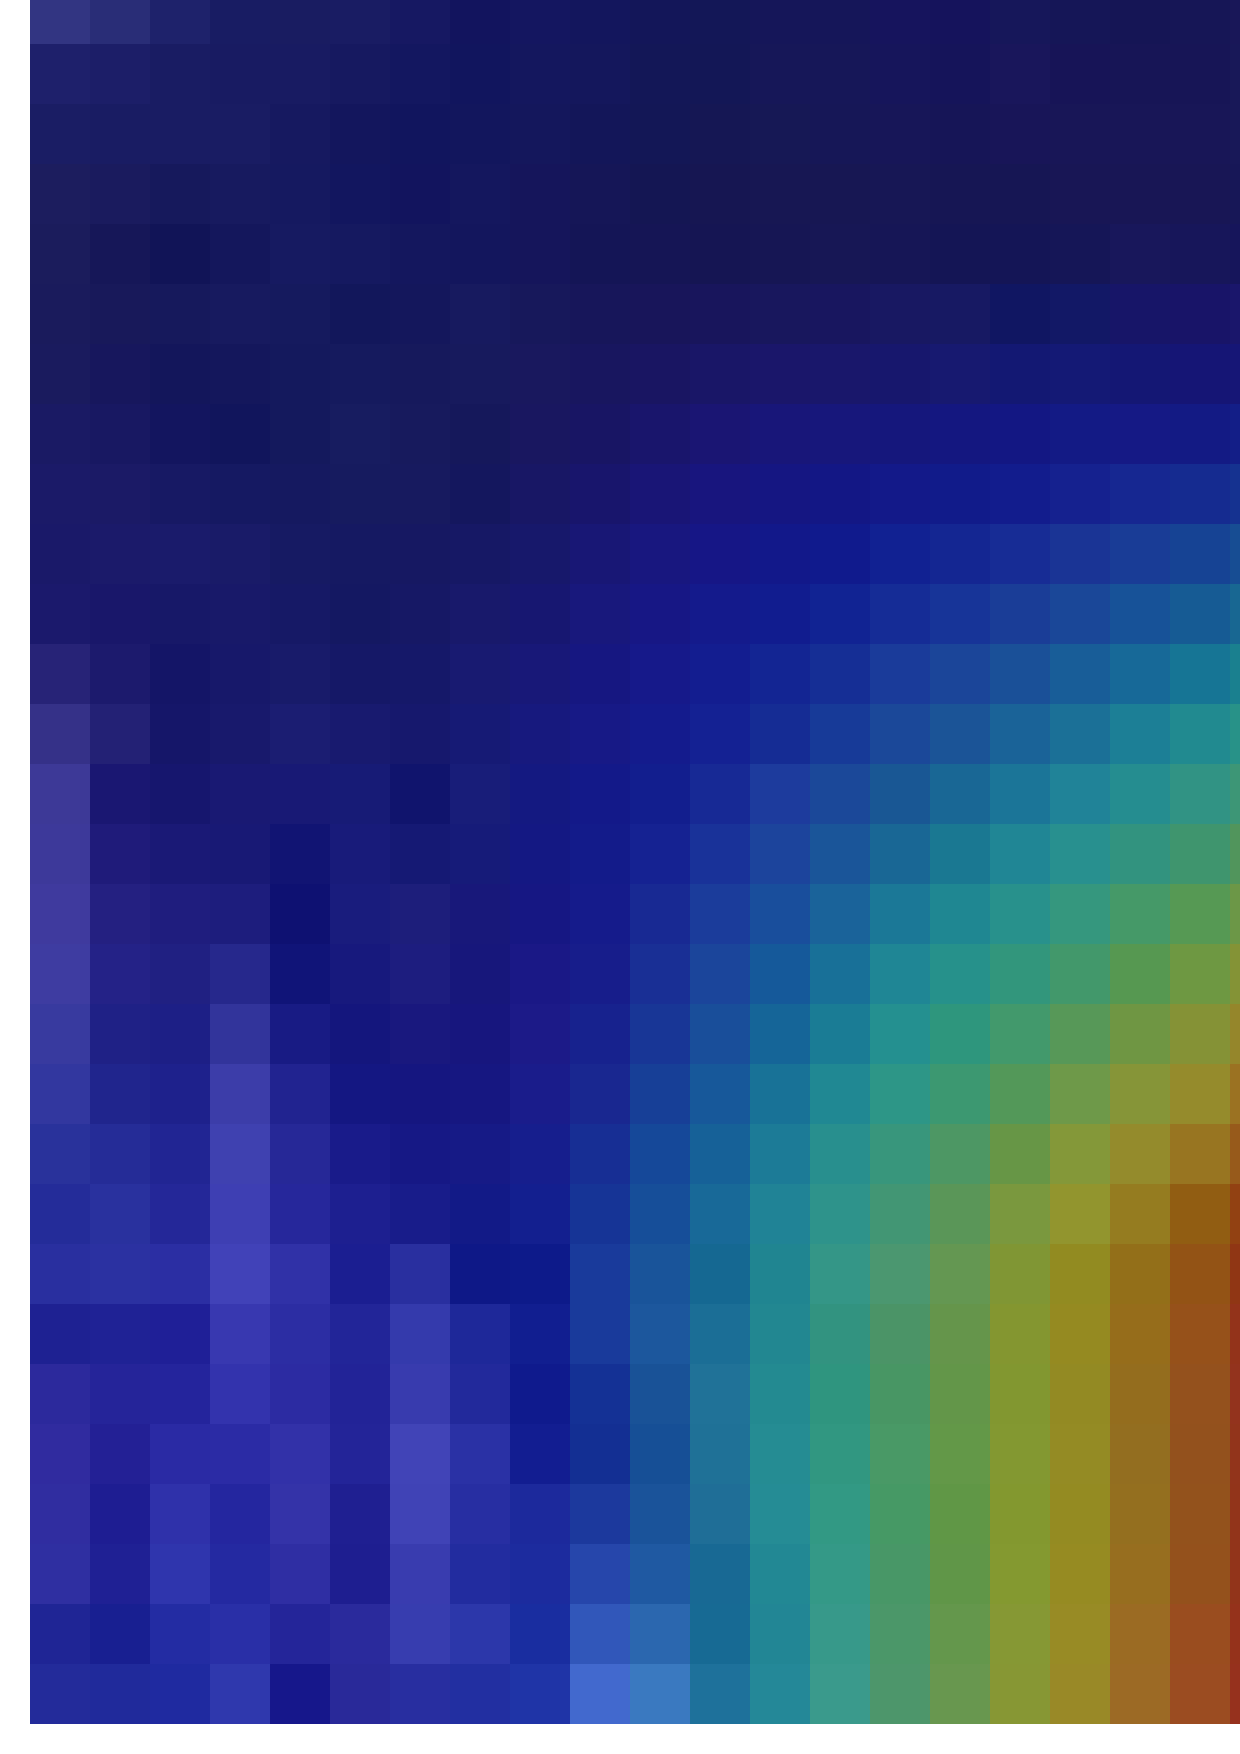
\includegraphics[scale=.015]{mask_nose_mouth.pdf}
	\caption{Grad-Cam on mask nose mouth class}
	\label{mask_nose_mouth}
\end{figure}

\begin{figure}[!b]
	\centering
	
\includegraphics[scale=.015]{mask_chin.pdf}
	\caption{Grad-Cam on mask chin class}
	\label{mask_chin}
\end{figure}


\section{Conclusion}

Based on the research results on the classification of how to use masks using the vision transformer architecture and data augmentation, it can be concluded that the implementation is carried out by performing RandAugment, on each existing dataset. Vision Transformer architecture is then applied by solving the digital image according to the number of patches that have been determined. Next will be a linear projection of the digital image so that the digital image will change the shape of the digital image from 3 dimensions to 2 dimensions. Then embedding will be carried out before entering the encoder transformer, where attention will be paid to the critical features in the digital image, which will eventually enter into the multi-layer perceptron, to be classified according to the existing class. The accuracy of the classification mask usage using ViT and data augmentation obtained accuracy results of 0.938462 for the Mask class, 0.761905 for the Mask Chin, 0.862682 for the Mask Mouth Chin class, and 0.725 for the Mask Nose Mouth class. Overall, the accuracy of the test data is 0.953383.


\bibliographystyle{unsrt}
%\bibliography{references}  %%% Remove comment to use the external .bib file (using bibtex).
%%% and comment out the ``thebibliography'' section.


%%% Comment out this section when you \bibliography{references} is enabled.
\begin{thebibliography}{1}

	\bibitem{Fortunato2010}Fortunato, S. Community detection in graphs. {\em Phys. Rep.-Rev. Sec. Phys. Lett.}. \textbf{486} pp. 75-174 (2010)
	\bibitem{NewmanGirvan2004}Newman, M. \& Girvan, M. Finding and evaluating community structure in networks. {\em Phys. Rev. E.}. \textbf{69} pp. 026113 (2004)
	\bibitem{Vehlowetal2013}Vehlow, C., Reinhardt, T. \& Weiskopf, D. Visualizing Fuzzy Overlapping Communities in Networks. {\em IEEE Trans. Vis. Comput. Graph.}. \textbf{19} pp. 2486-2495 (2013)
	\bibitem{Raghavanetal2007}Raghavan, U., Albert, R. \& Kumara, S. Near linear time algorithm to detect community structures in large-scale networks. {\em Phys. Rev E.}. \textbf{76} pp. 036106 (2007)
	\bibitem{SubeljBajec2011a}Šubelj, L. \& Bajec, M. Robust network community detection using balanced propagation. {\em Eur. Phys. J. B.}. \textbf{81} pp. 353-362 (2011)
	\bibitem{Louetal2013}Lou, H., Li, S. \& Zhao, Y. Detecting community structure using label propagation with weighted coherent neighborhood propinquity. {\em Physica A.}. \textbf{392} pp. 3095-3105 (2013)
	\bibitem{Clausetetal2004}Clauset, A., Newman, M. \& Moore, C. Finding community structure in very large networks. {\em Phys. Rev. E.}. \textbf{70} pp. 066111 (2004)
	\bibitem{Blondeletal2008}Blondel, V., Guillaume, J., Lambiotte, R. \& Lefebvre, E. Fast unfolding of communities in large networks. {\em J. Stat. Mech.-Theory Exp.}. \textbf{2008} pp. P10008 (2008)
	\bibitem{SobolevskyCampari2014}Sobolevsky, S. \& Campari, R. General optimization technique for high-quality community detection in complex networks. {\em Phys. Rev. E.}. \textbf{90} pp. 012811 (2014)
	\bibitem{FortunatoBarthelemy2007}Fortunato, S. \& Barthelemy, M. Resolution limit in community detection. {\em Proc. Natl. Acad. Sci. U. S. A.}. \textbf{104} pp. 36-41 (2007)
	\bibitem{SubeljBajec2011b}Šubelj, L. \& Bajec, M. Unfolding communities in large complex networks: Combining defensive and offensive label propagation for core extraction. {\em Phys. Rev. E.}. \textbf{83} pp. 036103 (2011)
	\bibitem{WangLi2013}Wang, X. \& Li, J. Detecting communities by the core-vertex and intimate degree in complex networks. {\em Physica A.}. \textbf{392} pp. 2555-2563 (2013)
	\bibitem{Lietal2013}Li, J., Wang, X. \& Eustace, J. Detecting overlapping communities by seed community in weighted complex networks. {\em Physica A.}. \textbf{392} pp. 6125-6134 (2013)
	\bibitem{Fabioetal2013}Fabio, D., Fabio, D. \& Carlo, P. Profiling core-periphery network structure by random walkers. {\em Sci. Rep.}. \textbf{3} pp. 1467 (2013)
	\bibitem{Chenetal2013}Chen, Q., Wu, T. \& Fang, M. Detecting local community structure in complex networks based on local degree central nodes. {\em Physica A.}. \textbf{392} pp. 529-537 (2013)
	\bibitem{Zhangetal2007}Zhang, S., Wang, R. \& Zhang, X. Identification of overlapping community structure in complex networks using fuzzy c-means clustering. {\em Physica A.}. \textbf{374} pp. 483-490 (2007)
	\bibitem{Nepuszetal2008}Nepusz, T., Petróczi, A., Négyessy, L. \& Bazsó, F. Fuzzy communities and the concept of bridgeness in complex networks. {\em Phys. Rev. E.}. \textbf{77} pp. 016107 (2008)
	\bibitem{FabricioLiang2013}Fabricio, B. \& Liang, Z. Fuzzy community structure detection by particle competition and cooperation. {\em Soft Comput.}. \textbf{17} pp. 659-673 (2013)
	\bibitem{Sunetal2011}Sun, P., Gao, L. \& Han, S. Identification of overlapping and non-overlapping community structure by fuzzy clustering in complex networks. {\em Inf. Sci.}. \textbf{181} pp. 1060-1071 (2011)
	\bibitem{Wangetal2013}Wang, W., Liu, D., Liu, X. \& Pan, L. Fuzzy overlapping community detection based on local random walk and multidimensional scaling. {\em Physica A.}. \textbf{392} pp. 6578-6586 (2013)
	\bibitem{Psorakisetal2011}Psorakis, I., Roberts, S., Ebden, M. \& Sheldon, B. Overlapping community detection using Bayesian non-negative matrix factorization. {\em Phys. Rev. E.}. \textbf{83} pp. 066114 (2011)
	\bibitem{ZhangYeung2012}Zhang, Y. \& Yeung, D. Overlapping Community Detection via Bounded Nonnegative Matrix Tri-Factorization. {\em In Proc. ACM SIGKDD Conf.}. pp. 606-614 (2012)
	\bibitem{Liu2010}Liu, J. Fuzzy modularity and fuzzy community structure in networks. {\em Eur. Phys. J. B.}. \textbf{77} pp. 547-557 (2010)
	\bibitem{Havensetal2013}Havens, T., Bezdek, J., Leckie \& Palaniswami, M. A Soft Modularity Function For Detecting Fuzzy Communities in Social Networks. {\em IEEE Trans. Fuzzy Syst.}. \textbf{21} pp. 1170-1175 (2013)
	\bibitem{Newman2013}Newman, M. Network data. (http://www-personal.umich.edu/ mejn/netdata/,2013)
	\bibitem{SubeljBajec2012}Šubelj, L. \& Bajec, M. Ubiquitousness of link-density and link-pattern communities in real-world networks. {\em Eur. Phys. J. B.}. \textbf{85} pp. 1-11 (2012)
	\bibitem{Lancichinettietal2008}Lancichinetti, A., Fortunato, S. \& Radicchi, F. Benchmark graphs for testing community detection algorithms. {\em Phys. Rev. E.}. \textbf{78} pp. 046110 (2008)
	\bibitem{Liuetal2014}Liu, W., Pellegrini, M. \& Wang, X. Detecting Communities Based on Network Topology. {\em Sci. Rep.}. \textbf{4} pp. 5739 (2014)
	\bibitem{Danonetal2005}Danon, L., Diaz-Guilera, A., Duch, J. \& Arenas, A. Comparing community structure identification. {\em J. Stat. Mech.-Theory Exp.}. pp. P09008 (2005)
	\bibitem{Gregory2011}Gregory, S. Fuzzy overlapping communities in networks. {\em J. Stat. Mech.-Theory Exp.}. pp. P02017 (2011)
	\bibitem{LancichinettiFortunato2009}Lancichinetti, A. \& Fortunato, S. Benchmarks for testing community detection algorithms on directed and weighted graphs with overlapping communities. {\em Phys. Rev. E.}. \textbf{80} pp. 016118 (2009)
	\bibitem{HullermeierRifqi2009}Hullermeier, E. \& Rifqi, M. A Fuzzy Variant of the Rand Index for Comparing Clustering Structures. {\em In Proc. IFSA/EUSFLAT Conf.}. pp. 1294-1298 (2009)
	\bibitem{Selvaraju2020gradcam}Selvaraju, R., Das, A., Vedantam, R., Cogswell, M., Parikh, D. \& Batra, D. Grad-CAM: Why did you say that? Visual Explanations from Deep Networks via Gradient-based Localization. {\em CoRR}. \textbf{abs/1610.02391} (2016), http://arxiv.org/abs/1610.02391
	\bibitem{Shorten2019}Shorten, C. \& Khoshgoftaar, T. A survey on Image Data Augmentation for Deep Learning. {\em Journal Of Big Data}. \textbf{6} (2019), https://doi.org/10.1186/s40537-019-0197-0
	\bibitem{Vaswani2017}Vaswani, A., Shazeer, N., Parmar, N., Uszkoreit, J., Jones, L., Gomez, A., Kaiser, Ł. \& Polosukhin, I. Attention is all you need. {\em Advances In Neural Information Processing Systems}. \textbf{2017-Decem}, 5999-6009 (2017)
	\bibitem{Zhang2019}Zhang, S., Han, F., Liang, Z., Tan, J., Cao, W., Gao, Y., Pomeroy, M., Ng, K. \& Hou, W. An investigation of CNN models for differentiating malignant from benign lesions using small pathologically proven datasets. {\em Computerized Medical Imaging And Graphics}. \textbf{77} pp. 101645 (2019), https://doi.org/10.1016/j.compmedimag.2019.101645
	\bibitem{Barman2019}Barman, R., Deshpande, S., Agarwal, S. \& Inamdar, U. Transfer Learning for Small Dataset. {\em National Conference On Machine Learning}. (2019), https://www.researchgate.net/publication/332407279_Transfer_Learning_for_Small_Dataset
	\bibitem{Soman2012}Soman, S., Ghorpade, M. \& Sonone, V. Content Based Image Retrieval using Color and Texture. {\em International Conference In Computational Intelligence (ICCIA)}. \textbf{3}, 39-57 (2012)
	\bibitem{Choi2019}Choi, D., Shallue, C., Nado, Z., Lee, J., Maddison, C. \& Dahl, G. On Empirical Comparisons of Optimizers for Deep Learning.  (2019), http://arxiv.org/abs/1910.05446
	\bibitem{Matsugu2003}Matsugu, M., Mori, K., Mitari, Y. \& Kaneda, Y. Subject independent facial expression recognition with robust face detection using a convolutional neural network. {\em Neural Networks}. \textbf{16}, 555-559 (2003)
	\bibitem{monteiro_cannon_moubarac_levy_louzada_jaime_2018}Monteiro, C., Cannon, G., Moubarac, J., Levy, R., Louzada, M. \& Jaime, P. The UN Decade of Nutrition, the NOVA food classification and the trouble with ultra-processing. {\em Public Health Nutrition}. \textbf{21}, 5-17 (2018)
	\bibitem{eka2013rahasia}Eka, R. \& Mariana, R. Rahasia Mengetahui Makanan Berbahaya. (Guepedia,2013), https://books.google.co.id/books?id=JJvRDgAAQBAJ
	\bibitem{Tomas2021}Tomás, J., Rego, A., Viciano-Tudela, S. \& Lloret, J. Incorrect Facemask-Wearing Detection Using Convolutional Neural Networks with Transfer Learning. {\em Healthcare}. \textbf{9}, 1050 (2021)
	\bibitem{Bosheng2020}Bosheng, Q. \& Li, D. Identifying Facemask-Wearing Condition Using Image Super-Resolution with Classification Network. {\em Mdpi Sensor}. pp. 1-23 (2020)
	\bibitem{Dosovitskiy2020}Dosovitskiy, A., Beyer, L., Kolesnikov, A., Weissenborn, D., Zhai, X., Unterthiner, T., Dehghani, M., Minderer, M., Heigold, G., Gelly, S., Uszkoreit, J. \& Houlsby, N. An Image is Worth 16x16 Words: Transformers for Image Recognition at Scale.  (2020), http://arxiv.org/abs/2010.11929
	\bibitem{C2020}C, M. Image resizing recipes in Pillow.  (2020), https://www.pythoninformer.com/python-libraries/pillow/imageops-resizing/
	\bibitem{Vasilev2019}Vasilev, I., Slater, D., Spacagna, G., Roelants, P. \& Zocca, V. Python Deep Learning 2nd. {\em Packt}. \textbf{2} pp. 92-96 (2019)
	\bibitem{Fei-Fei2010}Fei-Fei, L., Deng, J. \& Li, K. ImageNet: Constructing a large-scale image database. {\em Journal Of Vision}. \textbf{9}, 1037-1037 (2010)
	\bibitem{Weiss2016}Weiss, K., Khoshgoftaar, T. \& Wang, D. A survey of transfer learning. {\em Journal Of Big Data}. \textbf{3} (2016)
	\bibitem{Ba2016}Ba, J., Kiros, J. \& Hinton, G. Layer Normalization.  (2016), http://arxiv.org/abs/1607.06450
	\bibitem{Hendrycks2016}Hendrycks, D. \& Gimpel, K. Gaussian Error Linear Units (GELUs).  (2016), http://arxiv.org/abs/1606.08415
	\bibitem{Liu2017}Liu, D. A Practical Guide to ReLU.  (2017), https://medium.com/@danqing/a-practical-guide-to-relu-b83ca804f1f7
	\bibitem{Goodfellow-et-al-2016}Goodfellow, I., Bengio, Y. \& Courville, A. Deep Learning. (MIT Press,2016)
	\bibitem{Huang2017}Huang, G., Liu, Z., Van Der Maaten, L. \& Weinberger, K. Densely connected convolutional networks. {\em Proceedings - 30th IEEE Conference On Computer Vision And Pattern Recognition, CVPR 2017}. \textbf{2017-Janua} pp. 2261-2269 (2017)
	\bibitem{Andono2017}Andono, P., Sujoto, T. \& Muljono Pengolahan Citra Digital. (Penerbit Andi,2017)
	\bibitem{9259904}Memiş, S., Arslan, B., Batur, O. \& Sönmez, E. A Comparative Study of Deep Learning Methods on Food Classification Problem. {\em 2020 Innovations In Intelligent Systems And Applications Conference (ASYU)}. pp. 1-4 (2020)
	\bibitem{Brownlee2017}Brownlee, J. A Gentle Introduction to Backpropagation Through Time.  (2017), https://machinelearningmastery.com/gentle-introduction-backpropagation-time/
	\bibitem{9031051}Rajayogi, J., Manjunath, G. \& Shobha, G. Indian Food Image Classification with Transfer Learning. {\em 2019 4th International Conference On Computational Systems And Information Technology For Sustainable Solution (CSITSS)}. \textbf{4} pp. 1-4 (2019)
	\bibitem{Dawani2020}Dawani, J. Hands-On Mathematics for. (Packt Publishing Ltd,2020)
	\bibitem{ShivajiraoShinde2011}Shivajirao Shinde, B. The Origins of Digital Image Processing & Application areas in Digital Image Processing Medical Images. {\em IOSR Journal Of Engineering}. \textbf{1}, 66-71 (2011)
	\bibitem{GUBUR}GÜBÜR, K. How to Resize Images with Python in Bulk. , https://www.holisticseo.digital/python-seo/resize-image/
	\bibitem{Vu2020}Vu, C. Do and don't when using transformation to improve CNN deep learning model.  (2020), https://towardsdatascience.com/improves-cnn-performance-by-applying-data-transformation-bf86b3f4cef4
	\bibitem{Geron2018}Géron, A. Hands-on Machine Learning with Scikit-Learn, Keras, and Tensorflow, 2nd edition. (O'reilly,2018)
	\bibitem{Oumina2020}Oumina, A., El Makhfi, N. \& Hamdi, M. Control the COVID-19 Pandemic: Face Mask Detection Using Transfer Learning. {\em 2020 IEEE 2nd International Conference On Electronics, Control, Optimization And Computer Science, ICECOCS 2020}. pp. 22-26 (2020)
	\bibitem{Graham2021}Graham, B., El-Nouby, A., Touvron, H., Stock, P., Joulin, A., Jégou, H. \& Douze, M. LeViT: a Vision Transformer in ConvNet's Clothing for Faster Inference.  (2021), http://arxiv.org/abs/2104.01136
	\bibitem{tan2019efficientnet}Tan, M. \& Le, Q. EfficientNet: Rethinking Model Scaling for Convolutional Neural Networks. {\em CoRR}. \textbf{abs/1905.11946} (2019), http://arxiv.org/abs/1905.11946
	\bibitem{Wang2021}Wang, B., Zhao, Y. \& Chen, C. Hybrid Transfer Learning and Broad Learning System for Wearing Mask Detection in the COVID-19 Era. {\em IEEE Transactions On Instrumentation And Measurement}. \textbf{70} (2021)
	\bibitem{Russakovsky2015}Russakovsky, O., Deng, J., Su, H., Krause, J., Satheesh, S., Ma, S., Huang, Z., Karpathy, A., Khosla, A., Bernstein, M., Berg, A. \& Fei-Fei, L. ImageNet Large Scale Visual Recognition Challenge. {\em International Journal Of Computer Vision}. \textbf{115}, 211-252 (2015)
	\bibitem{Wang2016}Wang, J. \& Perez, L. The Effectiveness of Data Augmentation in Image Classification using Deep Learning Jason. {\em International Geoscience And Remote Sensing Symposium (IGARSS)}. \textbf{2016-Novem} pp. 5079-5082 (2016)
	\bibitem{Machida2020}Machida, M., Nakamura, I., Saito, R., Nakaya, T., Hanibuchi, T., Takamiya, T., Odagiri, Y., Fukushima, N., Kikuchi, H., Amagasa, S., Kojima, T., Watanabe, H. \& Inoue, S. Incorrect use of face masks during the current COVID-19 pandemic among the general public in Japan. {\em International Journal Of Environmental Research And Public Health}. \textbf{17}, 1-11 (2020)
	\bibitem{Cowling2010}Cowling, B., Zhou, Y., Ip, D., Leung, G. \& Aiello, A. Face masks to prevent transmission of influenza virus: a systematic review. {\em Epidemiology And Infection}. \textbf{138}, 449-456 (2010)
	\bibitem{WorldHealthOrganization2020}World Health Organization Mask use in the context of COVID-19. {\em World Health Organization}., 1-10 (2020), https://www.who.int/publications/i/item/advice-on-the-use-of-masks-in-the-community-during-home-care-and-in-healthcare-settings-in-the-context-of-the-novel-coronavirus-(2019-ncov)-outbreak
	\bibitem{Feng2020}Feng, S., Shen, C., Xia, N., Song, W., Fan, M. \& Cowling, B. Rational use of face masks in the COVID-19 pandemic. {\em The Lancet Respiratory Medicine}. \textbf{8}, 434-436 (2020)
	\bibitem{VanDyke2020}Van Dyke, M., Rogers, T., Pevzner, E., Satterwhite, C., Shah, H., Beckman, W., Farah Ahmed, ;., Charles, ;. \& Rule, ;. Morbidity and Mortality Weekly Report Trends in County-Level COVID-19 Incidence in Counties With and Without a Mask Mandate-Kansas, June 1-August 23, 2020.  (2020), https://www.cdc.gov/coronavirus/2019-ncov/prevent-
	\bibitem{Brienen2010}Brienen, N., Timen, A., Wallinga, J., Van Steenbergen, J. \& Teunis, P. The effect of mask use on the spread of influenza during a pandemic. {\em Risk Analysis}. \textbf{30}, 1210-1218 (2010)
	\bibitem{WHO2020}Who Anjuran mengenai penggunaan masker dalam konteks COVID-19. {\em World Health Organization}., 1-17 (2020), https://www.who.int/docs/default-source/searo/indonesia/covid19/anjuran-mengenai-penggunaan-masker-dalam-konteks-covid-19-june-20.pdf?sfvrsn=d1327a85_2
	\bibitem{Dwirusman2020}Dwirusman, C. Peran Dan Efektivitas Masker Dalam Pencegahan Penularan Corona Virus Disease 2019 (Covid-19). {\em Jurnal Medika Hutama}. \textbf{2}, 412-420 (2020)
	\bibitem{Wang2016a}Wang, Z., Liu, Z. \& Zheng, C. Introduction to neural networks. {\em Studies In Systems, Decision And Control}. \textbf{34} pp. 1-36 (2016)
	\bibitem{Chua2020}Chua, M., Cheng, W., Goh, S., Kong, J., Li, B., Lim, J., Mao, L., Wang, S., Xue, K., Yang, L., Ye, E., Zhang, K., Cheong, W., Tan, B., Li, Z., Tan, B. \& Loh, X. Face Masks in the New COVID-19 Normal: Materials, Testing, and Perspectives. {\em Research}. \textbf{2020} pp. 1-40 (2020)
	\bibitem{Rahim2020}Rahim, A., Kusrini, K. \& Luthfi, E. Convolutional Neural Network untuk Kalasifikasi Penggunaan Masker. {\em Inspiration: Jurnal Teknologi Informasi Dan Komunikasi}. \textbf{10}, 109 (2020)
	\bibitem{Ahmad2019}Ahmad, J., Farman, H. \& Jan, Z. Deep Learning Methods and Applications. {\em SpringerBriefs In Computer Science}. pp. 31-42 (2019)
	\bibitem{Putri2020}Putri, S. Studi Literatur: Efektivitas Penggunaan Masker Kain dalam Pencegahan Transmisi Covid-19. {\em Jurnal Kesehatan Manarang}. \textbf{6}, 10 (2020)
	\bibitem{Tan2018}Tan, C., Sun, F., Kong, T., Zhang, W., Yang, C. \& Liu, C. A survey on deep transfer learning. {\em Lecture Notes In Computer Science (including Subseries Lecture Notes In Artificial Intelligence And Lecture Notes In Bioinformatics)}. \textbf{11141 Lncs} pp. 270-279 (2018)
	\bibitem{Budiman2021}Budiman, B. Pendeteksian Penggunaan Masker Wajah Dengan Metode Convolutional Neural Network. {\em Jurnal Ilmu Komputer Dan Sistem Informasi}. \textbf{Vol.9 No.1} (2021)
	\bibitem{Aggarwal2014}Aggarwal, C. Educational and software resources for data classification. {\em Data Classification: Algorithms And Applications}. pp. 657-665 (2014)
	\bibitem{Karras2019}Karras, T., Laine, S. \& Aila, T. A style-based generator architecture for generative adversarial networks. {\em Proceedings Of The IEEE Computer Society Conference On Computer Vision And Pattern Recognition}. \textbf{2019-June} pp. 4396-4405 (2019)
	\bibitem{Sari2020}Sari, Y., Maulana, L., Bihanda, Y., Maligan, J., Nur'Aini, N. \& Widyadhana, D. Leftovers Nutrition Prediction for Augmenting Smart Nutrition Box Prototype Feature Using Image Processing Approach and AFLE Algorithm. {\em 2020 3rd International Conference On Computer And Informatics Engineering, IC2IE 2020}. pp. 101-105 (2020)
	\bibitem{Cabani2021}Cabani, A., Hammoudi, K., Benhabiles, H. \& Melkemi, M. MaskedFace-Net – A dataset of correctly/incorrectly masked face images in the context of COVID-19. {\em Smart Health}. \textbf{19} pp. 1-5 (2021)
	\bibitem{Sari2020a}Sari, Y., Adinugroho, S. \& Maligan, J. Multi-food Recognition In Single Tray Box Image With Scarcity Data Using Convolutional Neural Network.  (2020)
	\bibitem{Maulana2020}Maulana, L., Bihanda, Y. \& Sari, Y. Color space and color channel selection on image segmentation of food images. {\em Register: Jurnal Ilmiah Teknologi Sistem Informasi}. \textbf{6}, 141-151 (2020)
	\bibitem{Sari2019}Sari, Y., Dewi, R., Maligan, J., Ananta, A. \& Adinugroho, S. Automatic Food Leftover Estimation in Tray Box Using Image Segmentation. {\em Proceedings Of 2019 4th International Conference On Sustainable Information Engineering And Technology, SIET 2019}. pp. 212-216 (2019)
	\bibitem{Thiodorus2021}Thiodorus, G. Perbandingan Model Convolutional Neural Network Dengan Metode Transfer Learning Untuk.  (2021)
	\bibitem{Sari2020b}Sari, Y., Maligan, J. \& Bihanda, Y. Multiple Food or Non-Food Detection in Single Tray Box Image using Fraction of Pixel Segmentation for Developing Smart Nutrition Box Prototype. {\em International Journal Of Innovative Technology And Exploring Engineering}. \textbf{9}, 132-136 (2020)
	\bibitem{Sari2020c}Sari, Y., Dewi, R., Maligan, J., Maulana, L. \& Adinugroho, S. Automatic Leftover Weight Prediction in Tray Box Using Improved Image Segmentation Color Lighting Component. {\em Journal Of Southwest Jiaotong University}. \textbf{55}, 1-18 (2020)
	\bibitem{Sari2019a}Sari, Y., Dewi, R., Maligan, J., Ananta, A. \& Adinugroho, S. Automatic Food Leftover Estimation in Tray Box Using Image Segmentation. {\em Proceedings Of 2019 4th International Conference On Sustainable Information Engineering And Technology, SIET 2019}. pp. 212-216 (2019)
	\bibitem{Sari2020d}Sari, Y., Maligan, J. \& Prakoso, A. Improving the Elementary Leftover Food Estimation Algorithm by Using Clustering Image Segmentation in Nutrition Intake Problem. {\em CENIM 2020 - Proceeding: International Conference On Computer Engineering, Network, And Intelligent Multimedia 2020}. pp. 435-439 (2020)
	\bibitem{Nuraini2020}Nur'aini, N., Widyadhana, D., Bihanda, Y., Sari, Y. \& Maligan, J. Aplikasi Smart Nutrition Box dalam Identifikasi Kehilangan Zat Gizi (Loss of Nutrition) pada Limbah Makanan Kantin. {\em Jurnal Keteknikan Pertanian Tropis Dan Biosistem}. \textbf{8}, 275-283 (2020)
	\bibitem{cubuk2019randaugment}Cubuk, E., Zoph, B., Shlens, J. \& Le, Q. RandAugment: Practical automated data augmentation with a reduced search space.  (2019)
	\bibitem{he2015resnet}He, K., Zhang, X., Ren, S. \& Sun, J. Deep Residual Learning for Image Recognition. {\em CoRR}. \textbf{abs/1512.03385} (2015), http://arxiv.org/abs/1512.03385
	\bibitem{shahinfar2020datasize}Shahinfar, S., Meek, P. \& Falzon, G. How many images do I need? Understanding how sample size per class affects deep learning model performance metrics for balanced designs in autonomous wildlife monitoring. {\em CoRR}. \textbf{abs/2010.08186} (2020), https://arxiv.org/abs/2010.08186
	\bibitem{lecun1998cnn}Lecun, Y., Bottou, L., Bengio, Y. \& Haffner, P. Gradient-based learning applied to document recognition. {\em Proceedings Of The IEEE}. \textbf{86}, 2278-2324 (1998)
	\bibitem{alom2019datasetsize}Alom, M., Taha, T., Yakopcic, C., Westberg, S., Sidike, P., Nasrin, M., Hasan, M., Essen, B., Awwal, A. \& Asari, V. A State-of-the-Art Survey on Deep Learning Theory and Architectures. {\em Electronics}. \textbf{8} pp. 292 (2019,3)
	\bibitem{szegedey2014inception}Szegedy, C., Liu, W., Jia, Y., Sermanet, P., Reed, S., Anguelov, D., Erhan, D., Vanhoucke, V. \& Rabinovich, A. Going Deeper with Convolutions. {\em CoRR}. \textbf{abs/1409.4842} (2014), http://arxiv.org/abs/1409.4842
	\bibitem{simonyan15vgg}Simonyan, K. \& Zisserman, A. Very Deep Convolutional Networks for Large-Scale Image Recognition. {\em International Conference On Learning Representations}. (2015)
	\bibitem{alzubaidi2021surveycnn}Alzubaidi, L., Zhang, J., Humaidi, A., Al-Dujaili, A., Duan, Y., Al-Shamma, O., Santamarı́a, J., Fadhel, M., Al-Amidie, M. \& Farhan, L. Review of deep learning: concepts, CNN architectures, challenges, applications, future directions. {\em Journal Of Big Data}. \textbf{8} (2021,3), https://doi.org/10.1186/s40537-021-00444-8
	\bibitem{deng2009imagenet}Deng, J., Dong, W., Socher, R., Li, L., Li, K. \& Fei-Fei, L. Imagenet: A large-scale hierarchical image database. {\em 2009 IEEE Conference On Computer Vision And Pattern Recognition}. pp. 248-255 (2009)
	\bibitem{hendrycks2016gelu}Hendrycks, D. \& Gimpel, K. Bridging Nonlinearities and Stochastic Regularizers with Gaussian Error Linear Units. {\em CoRR}. \textbf{abs/1606.08415} (2016), http://arxiv.org/abs/1606.08415
	\bibitem{karras2018gan}Karras, T., Laine, S. \& Aila, T. A Style-Based Generator Architecture for Generative Adversarial Networks. {\em CoRR}. \textbf{abs/1812.04948} (2018), http://arxiv.org/abs/1812.04948
	\bibitem{ba2016layer}Ba, J., Kiros, J. \& Hinton, G. Layer Normalization.  (2016)
	\bibitem{howard2017mobilenets}Howard, A., Zhu, M., Chen, B., Kalenichenko, D., Wang, W., Weyand, T., Andreetto, M. \& Adam, H. MobileNets: Efficient Convolutional Neural Networks for Mobile Vision Applications.  (2017)
	\bibitem{Sarker2021realworldapplications}Sarker, I. Machine Learning: Algorithms, Real-World Applications and Research Directions. {\em SN Computer Science}. \textbf{2} (2021,3), https://doi.org/10.1007/s42979-021-00592-x
	\bibitem{Loey2021maskdetection}Loey, M., Manogaran, G., Taha, M. \& Khalifa, N. A hybrid deep transfer learning model with machine learning methods for face mask detection in the era of the COVID-19 pandemic. {\em Measurement}. \textbf{167} pp. 108288 (2021,1), https://doi.org/10.1016/j.measurement.2020.108288
	\bibitem{Cristianini2008svm}Cristianini, N. \& Ricci, E. Support Vector Machines. {\em Encyclopedia Of Algorithms}. pp. 928-932 (2008), https://doi.org/10.1007/978-0-387-30162-4_415
	\bibitem{wang2020RMFD}Wang, Z., Wang, G., Huang, B., Xiong, Z., Hong, Q., Wu, H., Yi, P., Jiang, K., Wang, N., Pei, Y., Chen, H., Miao, Y., Huang, Z. \& Liang, J. Masked Face Recognition Dataset and Application. {\em CoRR}. \textbf{abs/2003.09093} (2020), https://arxiv.org/abs/2003.09093
	\bibitem{kawulok2016advances}Kawulok, M., Celebi, E. \& Smolka, B. Advances in face detection and facial image analysis. (Springer,2016)
	\bibitem{breiman1984decisiiontree}Breiman, L., Friedman, J., Stone, C. \& Olshen, R. Classification and Regression Trees. (Taylor & Francis,1984), https://books.google.co.id/books?id=JwQx-WOmSyQC
	\bibitem{zhang2012ensemble}Zhang, C. \& Ma, Y. Ensemble machine learning: methods and applications. (Springer,2012)
	\bibitem{Loey2021NovelDeep}Loey, M., Manogaran, G., Taha, M. \& Khalifa, N. Fighting against COVID-19: A novel deep learning model based on YOLO-v2 with ResNet-50 for medical face mask detection. {\em Sustainable Cities And Society}. \textbf{65} pp. 102600 (2021,2), https://doi.org/10.1016/j.scs.2020.102600
	\bibitem{redmon2015yolo}Redmon, J., Divvala, S., Girshick, R. \& Farhadi, A. You Only Look Once: Unified, Real-Time Object Detection. {\em CoRR}. \textbf{abs/1506.02640} (2015), http://arxiv.org/abs/1506.02640
	\bibitem{Li2012annotated}Xiao-LI, Chao-SUN, LU, P., Xiao-WANG \& Yi-ZHONG Simultaneous image classification and annotation based on probabilistic model. {\em The Journal Of China Universities Of Posts And Telecommunications}. \textbf{19}, 107-115 (2012), https://www.sciencedirect.com/science/article/pii/S1005888511602549
	\bibitem{Hopfield1982rnn}Hopfield, J. Neural networks and physical systems with emergent collective computational abilities. {\em Proceedings Of The National Academy Of Sciences}. \textbf{79}, 2554-2558 (1982), https://www.pnas.org/content/79/8/2554
	\bibitem{hocreiter1997lstm}Hochreiter, S. \& Schmidhuber, J. Long Short-Term Memory. {\em Neural Computation}. \textbf{9}, 1735-1780 (1997,11), https://doi.org/10.1162/neco.1997.9.8.1735
	\bibitem{cubuk2018autoaugment}Cubuk, E., Zoph, B., Mané, D., Vasudevan, V. \& Le, Q. AutoAugment: Learning Augmentation Policies from Data. {\em CoRR}. \textbf{abs/1805.09501} (2018), http://arxiv.org/abs/1805.09501
	\bibitem{yampolskiy2019unexplainable}Yampolskiy, R. Unexplainability and Incomprehensibility of Artificial Intelligence. {\em CoRR}. \textbf{abs/1907.03869} (2019), http://arxiv.org/abs/1907.03869
	\bibitem{jacobgilpytorchcam}Gildenblat, J. \& Contributors PyTorch library for CAM methods. (GitHub,2021), https://github.com/jacobgil/pytorch-grad-cam
	\bibitem{agarap2018relu}Agarap, A. Deep Learning using Rectified Linear Units (ReLU). {\em CoRR}. \textbf{abs/1803.08375} (2018), http://arxiv.org/abs/1803.08375
	\bibitem{zhang2018crossentropy}Zhang, Z. \& Sabuncu, M. Generalized Cross Entropy Loss for Training Deep Neural Networks with Noisy Labels. {\em CoRR}. \textbf{abs/1805.07836} (2018), http://arxiv.org/abs/1805.07836
	\bibitem{novanto2020}Bayu Rahayudi, N. Deteksi Covid-19 pada Citra Sinar-X Dada Menggunakan Deep Learning yang Efisien. {\em Jurnal Teknologi Informasi Dan Ilmu Komputer}. \textbf{7}, 1289-1296 (2020), https://jtiik.ub.ac.id/index.php/jtiik/article/view/3651
	\bibitem{fadhil2020}Rahadika, F., Yudistira, N. \& Sari, Y. Facial Expression Recognition using Residual Convnet with Image Augmentations. {\em Jurnal Ilmu Komputer Dan Informasi}. \textbf{14}, 127-135 (2021), https://jiki.cs.ui.ac.id/index.php/jiki/article/view/968


\end{thebibliography}


\end{document}
